\section{Đề thi thử THPTQG Sở GD\&ĐT Thanh Hóa 25--26, Lần 1}
\vspace{-0.5cm}

\Opensolutionfile{ans}[ans/ans-45-26-2-ThanhHoa-YenDinh1-L1]
\caulc
%%%%%-----Câu 1-----%%%%%
\begin{ex}%[Sở GD\&ĐT THANH HÓA, TRƯỜNG THPT YÊN ĐỊNH 1]%[Trần Tiến Sĩ, 26-2-DuAnDeTHPT-2025-2026]%[2D4N1-2]
	Nguyên hàm của hàm số $f(x) = x^4 + x^2$ là
	\choice
	{$x^4 + x^2 + C$}
	{$4x^3 + 2x + C$}
	{\True $\dfrac{1}{5}x^5 + \dfrac{1}{3}x^3 + C$}
	{$x^5 + x^3 + C$}
	\loigiai{
		Ta có $\displaystyle\int f(x)\mathrm{\,d}x = \displaystyle\int \left(x^{4}+x^{2}\right)\mathrm{\,d}x = \dfrac{1}{5}x^{5}+\dfrac{1}{3}x^{3}+C$.
	}
\end{ex}

%%%%%-----Câu 2-----%%%%%
\begin{ex}%[Sở GD\&ĐT THANH HÓA, TRƯỜNG THPT YÊN ĐỊNH 1]%[Trần Tiến Sĩ, 26-2-DuAnDeTHPT-2025-2026]%[2H2N2-4]
	Trong không gian với hệ tọa độ $Oxyz$, cho vectơ $\vec{u} = (3;0;1)$. Độ dài của vectơ $\vec{u}$ bằng
	\choice
	{$\left|\vec{u}\right| = 3$}
	{$\left|\vec{u}\right| = 10$}
	{$\left|\vec{u}\right| = 4$}
	{\True $\left|\vec{u}\right| = \sqrt{10}$}
	\loigiai{
		Độ dài của vectơ $\left|\vec{u}\right|=\sqrt{3^{2}+0^{2}+1^{2}}=\sqrt{10}$.
	}
\end{ex}

%%%%%-----Câu 3-----%%%%%
\begin{ex}%[Sở GD\&ĐT THANH HÓA, TRƯỜNG THPT YÊN ĐỊNH 1]%[Trần Tiến Sĩ, 26-2-DuAnDeTHPT-2025-2026]%[2D1N2-2]
	Cho hàm số $y = f(x)$ có bảng xét dấu của đạo hàm như sau
	\begin{center}
		
\begin{tikzpicture}
			\tkzTabInit[nocadre=false,lgt=1.5,espcl=2,deltacl=0.6]
			{$x$ / 1, $f'(x)$ / 1}
			{$-\infty$, $-2$, $-1$, $1$, $4$, $+\infty$}
			\tkzTabLine{ , -, 0, +, 0, -, 0, +, 0,- }
		\end{tikzpicture}
	\end{center}
	Số điểm cực trị của hàm số đã cho là
	\choice
	{\True $4$}
	{$5$}
	{$3$}
	{$2$}
	\loigiai{
		Dựa vào bảng xét dấu, $f'(x)$ đổi dấu khi qua các điểm $x\in\left\{-2;-1;1;4\right\}$.
		Vậy số điểm cực trị của hàm số đã cho là $4$.
	}
\end{ex}

%%%%%-----Câu 4-----%%%%%
\begin{ex}%[Sở GD\&ĐT THANH HÓA, TRƯỜNG THPT YÊN ĐỊNH 1]%[Trần Tiến Sĩ, 26-2-DuAnDeTHPT-2025-2026]%[2H2N1-2]
	\immini{
		Cho hình chóp $S.ABCD$, có đáy $ABCD$ hình bình hành. Khẳng định nào sau đây đúng?
		\choice
		{$\vec{SB} - \vec{SA} + \vec{AD} = \vec{0}$}
		{$\vec{SB} - \vec{SA} + \vec{AD} = \vec{AB}$}
		{\True $\vec{SB} - \vec{SA} + \vec{AD} = \vec{AC}$}
		{$\vec{SB} - \vec{SA} + \vec{AD} = \vec{SC}$}
	}{
		\begin{tikzpicture}[line join=round, line cap=round, >=stealth, scale=0.8, font=\footnotesize]
			% Định nghĩa tọa độ các đỉnh đáy (Hình chữ nhật vẽ dạng hình bình hành)
			\coordinate (A) at (0,0);
			\coordinate (D) at (-1.5,-1.5);
			\coordinate (B) at (3,0);
			\coordinate (C) at ($(B)+(D)-(A)$);
			
			% Định nghĩa đỉnh S (SA vuông góc đáy)
			\coordinate (S) at (0.5,3);
			
			% Vẽ các nét đứt (cạnh khuất)
			\draw[dashed] (S)--(A);
			\draw[dashed] (A)--(B);
			\draw[dashed] (A)--(D);
			
			% Vẽ các nét liền (cạnh thấy)
			\draw (S)--(B);
			\draw (S)--(C); 
			\draw (S)--(D);
			\draw (B)--(C)--(D);
			
			% Gán nhãn các đỉnh
			\foreach \p/\anch in {S/above, A/above left, B/right, C/below right, D/below left} {
				\fill[black] (\p) circle (1.2pt);
				\node[\anch] at (\p) {$\p$};
			}			
		\end{tikzpicture}
	}
	
	\loigiai{
		Ta có $\vec{SB}-\vec{SA}=\vec{AB}$.
		Theo quy tắc hình bình hành $\vec{AB}+\vec{AD}=\vec{AC}$.\\
		Từ đó suy ra $\vec{SB}-\vec{SA}+\vec{AD}=\vec{AC}$.
	}
\end{ex}

%%%%%-----Câu 5-----%%%%%
\begin{ex}%[Sở GD\&ĐT THANH HÓA, TRƯỜNG THPT YÊN ĐỊNH 1]%[Trần Tiến Sĩ, 26-2-DuAnDeTHPT-2025-2026]%[2D3N1-2]
	Xét mẫu số liệu ghép nhóm như sau, trong đó $n_1 >0$ và $n_m >0$
	\begin{center}
		\begin{tabular}{|c|c|c|c|c|}
			\hline
			Nhóm  & $[a_1; a_2)$ & $[a_2; a_3)$ & $\dots$ & $[a_m; a_{m+1})$ \\ \hline
			Tần số &    $n_1$     &    $n_2$     & $\dots$ &      $n_m$       \\ \hline
		\end{tabular}
	\end{center}
	Khi đó, khoảng biến thiên của mẫu số liệu ghép nhóm trên là
	\choice
	{$R = a_{m+1} - a_m$}
	{\True $R = a_{m+1} - a_1$}
	{$R = a_m - a_1$}
	{$R = a_{m+1} - a_2$}
	\loigiai{
		Khoảng biến thiên của mẫu số liệu ghép nhóm là $R=a_{m+1}-a_{1}$.
	}
\end{ex}

%%%%%-----Câu 6-----%%%%%
\begin{ex}%[Sở GD\&ĐT THANH HÓA, TRƯỜNG THPT YÊN ĐỊNH 1]%[Trần Tiến Sĩ, 26-2-DuAnDeTHPT-2025-2026]%[2D4H2-1]
	Nếu $\displaystyle\int\limits_0^2 f(x) \mathrm{\,d}x = 3$ thì $\displaystyle\int\limits_0^2 \left[ 2x - f(x) \right] \mathrm{\,d}x$ bằng
	\choice
	{$-2$}
	{$7$}
	{\True $1$}
	{$10$}
	\loigiai{
		Ta có $\displaystyle\int\limits_{0}^{2}[2x-f(x)]\mathrm{\,d}x = \displaystyle\int\limits_{0}^{2}2x\mathrm{\,d}x - \displaystyle\int\limits_{0}^{2}f(x)\mathrm{\,d}x = \left. x^{2} \right|_{0}^{2} - 3 = 4 - 3 = 1$.
	}
\end{ex}

%%%%%-----Câu 7-----%%%%%
\begin{ex}%[Sở GD\&ĐT THANH HÓA, TRƯỜNG THPT YÊN ĐỊNH 1]%[Trần Tiến Sĩ, 26-2-DuAnDeTHPT-2025-2026]%[1H4H3-2]
	\immini{
		Cho hình hộp $ABCD.A'B'C'D'$ (xem hình bên). Đường thẳng $AB$ song song với mặt phẳng nào sau đây?
		\choice
		{\True $(A'B'C'D')$}
		{$(CC'A'A)$}
		{$(AA'D'D)$}
		{$(BB'C'C)$}
	}{
		\begin{tikzpicture}[line join=round, line cap=round, >=stealth, scale=0.75, font=\footnotesize]
			% Định nghĩa tọa độ các đỉnh đáy dưới ABCD (Hình bình hành)
			\coordinate (A) at (0,0);
			\coordinate (B) at (-1.5,-1.5);
			\coordinate (D) at (3,0);
			\coordinate (C) at ($(B)+(D)-(A)$);
			
			% Định nghĩa đỉnh A' bằng cách tịnh tiến đỉnh A (cạnh bên xiên)
			\coordinate (A') at (0.5,3);
			
			% Xác định các đỉnh còn lại của đáy trên bằng phép tịnh tiến vectơ AA'
			\coordinate (B') at ($(B)+(A')-(A)$);
			\coordinate (C') at ($(C)+(A')-(A)$);
			\coordinate (D') at ($(D)+(A')-(A)$);
			
			% Vẽ các nét đứt (cạnh khuất xuất phát từ đỉnh A)
			\draw[dashed] (A)--(B);
			\draw[dashed] (A)--(D);
			\draw[dashed] (A)--(A');
			
			% Vẽ các nét liền (các cạnh thấy)
			% Đáy trên
			\draw (A')--(B')--(C')--(D')--cycle;
			% Các cạnh bên
			\draw (B)--(B');
			\draw (C)--(C');
			\draw (D)--(D');
			% Phần thấy của đáy dưới
			\draw (B)--(C)--(D);
			
			% Gán nhãn các đỉnh
			\foreach \p/\anch in {
				A/above left, B/below left, C/below right, D/below right, 
				A'/above left, B'/above left, C'/below right, D'/above right} {
				\fill[black] (\p) circle (1.2pt);
				\node[\anch] at (\p) {$\p$};
			}            
		\end{tikzpicture}        
	}
	
	\loigiai{
		Đường thẳng $AB$ song song với đường thẳng $A'B'$, mà $A'B' \subset (A'B'C'D')$.\\
		Do đó đường thẳng $AB$ song song với mặt phẳng $(A'B'C'D')$.
	}
\end{ex}

%%%%%-----Câu 8-----%%%%%
\begin{ex}%[Sở GD\&ĐT THANH HÓA, TRƯỜNG THPT YÊN ĐỊNH 1]%[Trần Tiến Sĩ, 26-2-DuAnDeTHPT-2025-2026]%[1D6H4-4]
	Số nghiệm của phương trình $\log_3(x^2 + 4x) + \log_{\frac{1}{3}} 5 = 0$ là
	\choice
	{$0$}
	{$1$}
	{\True $2$}
	{$3$}
	\loigiai{
		Viết lại phương trình ta được
		\allowdisplaybreaks 
		\begin{eqnarray*} 
		\log_{3}(x^{2}+4x) = \log_{3}5 \Leftrightarrow \heva{&x^{2}+4x>0\\ &x^{2}+4x=5} \Leftrightarrow \hoac{&x=1\\ &x=-5.} 
		\end{eqnarray*} 
		Vậy phương trình có $2$ nghiệm.
	}
\end{ex}

%%%%%-----Câu 9-----%%%%%
\begin{ex}%[Sở GD\&ĐT THANH HÓA, TRƯỜNG THPT YÊN ĐỊNH 1]%[Trần Tiến Sĩ, 26-2-DuAnDeTHPT-2025-2026]%[2H2N2-3]
	Trong không gian với hệ tọa độ $Oxyz$, cho hai vectơ $\vec{a} = (1;1;0)$, $\vec{b} = (3;-1;0)$. Tọa độ vectơ $\vec{u} = 2\vec{a} - \vec{b}$ là
	\choice
	{$\vec{u} = (4;0;0)$}
	{$\vec{u} = (7;-1;0)$}
	{$\vec{u} = (1;-3;0)$}
	{\True $\vec{u} = (-1;3;0)$}
	\loigiai{
		Ta có $2\vec{a}-\vec{b} = 2(1;1;0) - (3;-1;0) = (-1;3;0)$.
		Suy ra $\vec{u}=(-1;3;0)$.
	}
\end{ex}

%%%%%-----Câu 10-----%%%%%
\begin{ex}%[Sở GD\&ĐT THANH HÓA, TRƯỜNG THPT YÊN ĐỊNH 1]%[Trần Tiến Sĩ, 26-2-DuAnDeTHPT-2025-2026]%[1D1N5-3]
	Tập nghiệm của phương trình $\sin x = 0$ là
	\choice
	{$S = \left\{k2\pi \ \middle| \ k \in \mathbb{Z}\right\}$}
	{$S = \left\{\dfrac{\pi}{2} + k\pi \ \middle| \ k \in \mathbb{Z}\right\}$}
	{\True $S = \left\{k\pi \ \middle| \ k \in \mathbb{Z}\right\}$}
	{$S = \left\{\dfrac{\pi}{2} + k2\pi \ \middle| \ k \in \mathbb{Z}\right\}$}
	\loigiai{
		Phương trình $\sin x = 0 \Leftrightarrow x = k\pi \ (k \in \mathbb{Z})$.
		Vậy tập nghiệm là $S=\left\{k\pi \ \middle| \ k\in\mathbb{Z}\right\}$.
	}
\end{ex}

%%%%%-----Câu 11-----%%%%%
\begin{ex}%[Sở GD\&ĐT THANH HÓA, TRƯỜNG THPT YÊN ĐỊNH 1]%[Trần Tiến Sĩ, 26-2-DuAnDeTHPT-2025-2026]%[1D2N3-2]
	Cho cấp số nhân $(u_n)$ với các số hạng $u_1 = -\dfrac{1}{2}; u_2 = 1$. Công bội $q$ của cấp số nhân là
	\choice
	{$q = \pm 2$}
	{\True $q = -2$}
	{$q = -\dfrac{33}{10}$}
	{$q = 2$}
	\loigiai{
		Ta có $u_{2}=u_{1} \cdot q $ nên $ 1 = \left(-\dfrac{1}{2}\right) \cdot q $ suy ra $ q=-2$.
	}
\end{ex}

%%%%%-----Câu 12-----%%%%%
\begin{ex}%[Sở GD\&ĐT THANH HÓA, TRƯỜNG THPT YÊN ĐỊNH 1]%[Trần Tiến Sĩ, 26-2-DuAnDeTHPT-2025-2026]%[2D1N1-2]
	Cho hàm số $y = f(x)$ xác định trên $\mathbb{R} \setminus \{-6\}$ và có bảng biến thiên như sau
	\begin{center}
		
\begin{tikzpicture}[double distance=4pt] 
			\tkzTabInit[nocadre=false,lgt=1.2,espcl=3,deltacl=0.6]
			{$x$ / 1, $y'$ / 1, $y$ / 2}
			{$-\infty$, $-7$, $-6$, $0$, $+\infty$}
			\tkzTabLine{ , -, 0, +, d, +, 0, -, }
			\tkzTabVar{+/ $+\infty$, -/ $-6$, +D-/ $+\infty$ / $-\infty$, +/ $-15$, -/ $-\infty$}
		\end{tikzpicture}
	\end{center}
	Hàm số $y = f(x)$ đồng biến trên khoảng nào trong các khoảng dưới đây?
	\choice
	{\True $(-7; -6)$}
	{$(-6; +\infty)$}
	{$(-10; 1)$}
	{$(0; +\infty)$}
	\loigiai{
		Dựa vào bảng biến thiên, ta thấy $y' > 0$ trên các khoảng $(-7;-6)$ và $(-6;0)$.\\
		Do đó, hàm số $y=f(x)$ đồng biến trên khoảng $(-7;-6)$.
	}
\end{ex}

\Closesolutionfile{ans}

\Opensolutionfile{ans}[ans/ans-45-26-2-ThanhHoa-YenDinh1-L1-DS]
\cauds
%%%%%-----Câu 1-----%%%%%
\begin{ex}%[Sở GD\&ĐT THANH HÓA, TRƯỜNG THPT YÊN ĐỊNH 1]%[Trần Tiến Sĩ, 26-2-DuAnDeTHPT-2025-2026]%[2D4V2-6]
	Một ô tô bắt đầu chuyển động thẳng nhanh dần đều với vận tốc $v(t) = 5t$ (m/s); trong đó $t$ là thời gian tính bằng giây kể từ khi ô tô bắt đầu chuyển động. Đi được $6$ (s) người lái xe phát hiện chướng ngại vật và phanh gấp, ô tô tiếp tục chuyển động chậm dần đều với gia tốc $a = -5$ (m/s$^2$).
	\choiceTF
	{Quãng đường ô tô chuyển động được trong $6$ giây đầu tiên là $80$ m}
	{\True Quãng đường $S$ (đơn vị: mét) mà ô tô chuyển động được kể từ lúc bắt đầu đạp phanh đến khi dừng lại được tính theo công thức $S = \displaystyle\int\limits_6^{12} (60 - 5t) \mathrm{\,d}t$}
	{\True Vận tốc của ô tô tại thời điểm $t = 6$ (s) là $30$ (m/s)}
	{Quãng đường ô tô chuyển động được kể từ lúc bắt đầu chuyển động cho đến khi dừng lại là $170$ m}
	\loigiai{
		\begin{itemchoice}
			\itemch Quãng đường ô tô chuyển động được trong $6$ giây đầu tiên là $S_{1}=\displaystyle\int\limits_{0}^{6} 5t \mathrm{\,d}t=90$ (m).
			\itemch Sau khi phanh gấp, ô tô chuyển động theo hàm vận tốc 
			\allowdisplaybreaks 
			\begin{eqnarray*} 
				v_{1}(t)=\displaystyle\int a \mathrm{\,d}t=\displaystyle\int(-5)\mathrm{\,d}t=-5t+C.
			\end{eqnarray*} 
			Tại thời điểm phanh $t=6$, ta có $v_1(6)=30 \Rightarrow C=60 \Rightarrow v_1(t) = -5t+60$.
			
			Thời điểm ô tô dừng lại là khi $v_1(t)=0 \Leftrightarrow t=12$.
			
			Do đó, quãng đường được tính bởi công thức $S=\displaystyle\int\limits_{6}^{12}(60-5t)\mathrm{\,d}t$.
			\itemch Ta có vận tốc tại thời điểm $t=6$ là $v(6)=5 \cdot 6=30$ (m/s).
			\itemch Quãng đường ô tô chuyển động kể từ lúc đạp phanh đến khi dừng lại là 
			\allowdisplaybreaks 
			\begin{eqnarray*} 
				S=\displaystyle\int\limits_{6}^{12}(60-5t)\mathrm{\,d}t=90 \, \text{(m)}.
			\end{eqnarray*} 
			Vậy tổng quãng đường ô tô đi được từ lúc bắt đầu đến khi dừng hẳn là $90+90=180$ (m).
		\end{itemchoice}
	}
\end{ex}

%%%%%-----Câu 2-----%%%%%
\begin{ex}%[Sở GD\&ĐT THANH HÓA, TRƯỜNG THPT YÊN ĐỊNH 1]%[Trần Tiến Sĩ, 26-2-DuAnDeTHPT-2025-2026]%[1D9H2-5]
	Khi khảo sát một nhóm học sinh có $50$ em về các môn thể thao các em yêu thích. Người ta thấy rằng có $31$ em thích chơi đá bóng, $12$ em thích chơi cầu lông, $5$ em vừa thích chơi đá bóng và vừa thích chơi cầu lông. Chọn ngẫu nhiên một học sinh trong nhóm học sinh đó.
	\choiceTF
	{Xác suất để học sinh đó thích chơi đá bóng và không thích chơi cầu lông bằng $\dfrac{12}{25}$}
	{\True Xác suất để học sinh đó thích chơi cầu lông là $\dfrac{6}{25}$}
	{Xác suất để học sinh đó thích chơi đá bóng là $\dfrac{19}{50}$}
	{\True Xác suất để học sinh đó thích chơi đá bóng hoặc thích chơi cầu lông bằng $\dfrac{19}{25}$}
	\loigiai{
		Gọi $A$ là biến cố ``Học sinh đó thích chơi đá bóng'', $B$ là biến cố ``Học sinh đó thích chơi cầu lông''. \\		
		Ta có $\mathrm{P}(A)=\dfrac{31}{50}$, $\mathrm{P}(B)=\dfrac{12}{50}$, $\mathrm{P}(AB)=\dfrac{5}{50}$.
		\begin{itemchoice}
			\itemch Xác suất học sinh thích đá bóng và không thích cầu lông là
			\allowdisplaybreaks 
			\begin{eqnarray*}
				\mathrm{P}(A\overline{B})=\mathrm{P}(A)-\mathrm{P}(AB)=\dfrac{31}{50}-\dfrac{5}{50}=\dfrac{13}{25}.
			\end{eqnarray*}
			\itemch Xác suất để học sinh đó thích chơi cầu lông là $\mathrm{P}(B)=\dfrac{12}{50}=\dfrac{6}{25}$.
			\itemch Xác suất để học sinh đó thích chơi đá bóng là $\mathrm{P}(A)=\dfrac{31}{50}$.
			\itemch Xác suất để học sinh đó thích chơi đá bóng hoặc thích chơi cầu lông là 
			\allowdisplaybreaks 
			\begin{eqnarray*} 
				\mathrm{P}(A\cup B)=\mathrm{P}(A)+\mathrm{P}(B)-\mathrm{P}(AB)=\dfrac{31}{50}+\dfrac{12}{50}-\dfrac{5}{50}=\dfrac{38}{50}=\dfrac{19}{25}.
			\end{eqnarray*} 
		\end{itemchoice}
	}
\end{ex}

%%%%%-----Câu 3-----%%%%%
\begin{ex}%[Sở GD\&ĐT THANH HÓA, TRƯỜNG THPT YÊN ĐỊNH 1]%[Trần Tiến Sĩ, 26-2-DuAnDeTHPT-2025-2026]%[2D1H5-4]
	Cho hàm số $y = \dfrac{x^2 + 2x - 1}{x + 1}$
	\choiceTF
	{Tập xác định $\mathscr{D} = \mathbb{R} \setminus \{1\}$}
	{Đạo hàm $y' = 0 \Leftrightarrow x = 1$}
	{\True Đồ thị hàm số cắt trục $Ox$ tại $(-1 - \sqrt{2}; 0)$, $(-1 + \sqrt{2}; 0)$}
	{\True Giá trị của hàm số tại $x = 1$ là $y = 1$}
	\loigiai{
		\begin{itemchoice}
			\itemch Điều kiện xác định $x+1\ne 0 \Leftrightarrow x\ne -1$. Tập xác định của hàm số là $\mathscr{D}=\mathbb{R}\setminus\{-1\}$.
			\itemch Ta có đạo hàm $y'=\dfrac{x^{2}+2x+3}{(x+1)^{2}}>0$ với mọi $x\in \mathscr{D}$, do đó phương trình $y'=0$ vô nghiệm.
			\itemch Xét phương trình hoành độ giao điểm với trục hoành
			\allowdisplaybreaks 
			\begin{eqnarray*} 
				\dfrac{x^{2}+2x-1}{x+1}=0 \Leftrightarrow\heva{&x^{2}+2x-1=0\\ &x\ne -1} \Leftrightarrow \hoac{&x=-1+\sqrt{2}\\ &x=-1-\sqrt{2}.}
			\end{eqnarray*} 
			\itemch Thay $x=1$ vào hàm số $y=\dfrac{x^{2}+2x-1}{x+1}$ ta được $y(1)=\dfrac{1^2+2\cdot 1-1}{1+1}=1$.
		\end{itemchoice}
	}
\end{ex}

%%%%%-----Câu 4-----%%%%%
\begin{ex}%[Sở GD\&ĐT THANH HÓA, TRƯỜNG THPT YÊN ĐỊNH 1]%[Trần Tiến Sĩ, 26-2-DuAnDeTHPT-2025-2026]%[2H5C3-4]
	\immini{
		Trong không gian $Oxyz$, một con chim bồ câu xuất phát từ $O(0;0;0)$ di chuyển với vectơ vận tốc $\vec{v_1} = (1;2;2)$. Cùng lúc đó, một con chim én cũng bắt đầu di chuyển từ $A(0;0;5)$ với vectơ vận tốc $\vec{v_2} = (0;3;4)$. Tồn tại một vùng không gian nguy hiểm, nơi mà người ta thường xuyên săn bắn chim có dạng mặt cầu $(S) \colon (x-2)^2 + (y-4)^2 + (z-4)^2 = 16$. Biết rằng đơn vị độ dài trên mỗi trục tọa độ là $1{,}5$ mét và đơn vị đo thời gian là giây.
	}{
		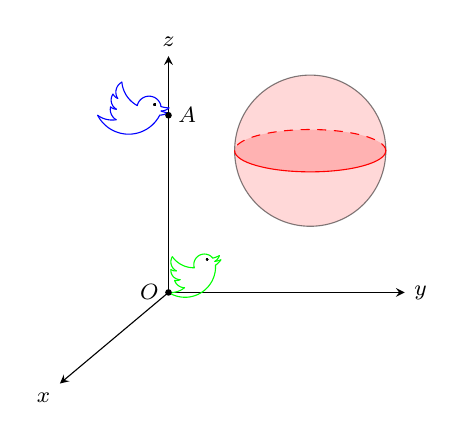
\begin{tikzpicture}[, line cap=round, line join=round, >=stealth, font=\footnotesize, scale=3]
			\tikzset{
				conchim/.pic={
					\foreach \x/\y/\A/\B/\R in {
						3.0000/4.6576/-2.1430/0.0508/5.5402,
						6.4847/7.9339/5.3122/5.6935/3.6285,
						7.7575/10.3789/4.8464/5.0847/4.7912,
						7.3921/7.2876/5.2578/5.9640/1.9381,
						7.0062/10.8271/4.9307/5.2050/4.7073,
						6.5160/5.0452/0.6660/3.4400/1.9201,
						4.5627/9.2001/3.7557/4.7374/4.7209,
						2.2429/5.5292/2.5882/4.2498/1.8084,
						1.2705/5.5530/4.1813/4.8128/1.6504,
						2.1092/4.0034/3.0662/4.7127/1.6794,
						1.3891/3.7137/4.5371/5.1907/1.5655,
						2.9180/2.7531/3.4534/4.7057/1.8931,
						0.4316/3.8797/4.6016/5.3987/3.9036%
					} {
						\draw[shift={(\x,\y)},] plot[domain=\A:\B, variable=\t] ({\R*cos(\t r)}, {\R*sin(\t r)});
						\fill[black] (7,6) circle (6pt);
					}
				}
			}
			% VẼ HỆ TRỤC TỌA ĐỘ
			\coordinate (O') at (0,0);
			\coordinate (A) at (0,0.75);
			\draw[->] (O') -- (-140:0.6) node[below left] {$x$};
			\draw[->] (O') -- (1, 0) node[right] {$y$};
			\draw[->] (O') -- (0, 1) node[above] {$z$};
			
			% Chèn con chim 
			\path (-0.3,0.75) pic[scale=0.08, color=blue, rotate=-30] {conchim};
			\path (O') pic[scale=0.07, color=green, rotate=0] {conchim};
			\fill[black] (A) circle (0.4pt);
			\fill[black] (O') circle (0.4pt);
			\node[left] (O') {$O$};
			\node[right] at (0,0.75) {$A$};
			
			% Đặt toàn bộ khối cầu vào một scope và tịnh tiến
			\begin{scope}[shift={(0.6,0.6)}, scale=0.32]
				% Tâm O lúc này cục bộ 
				\coordinate (O) at (0,0);
				
				% VẼ MẶT PHẲNG Oxy VÀ MẶT CẦU BẰNG ELIP & ĐƯỜNG TRÒN
				\fill[red!30] (O) ellipse (1 and 0.28);
				\draw[fill=red!30, opacity=0.5] (O) circle (1);
				
				\draw[dashed, red] (1,0) arc (0:180:1 and 0.28);
				\draw[red] (1,0) arc (0:-180:1 and 0.28);
			\end{scope}
		\end{tikzpicture}
	}
	\choiceTF
	{\True Tốc độ di chuyển của chim bồ câu là $4{,}5$ (m/s)}
	{\True Chim én và chim bồ câu không va chạm nhau trong quá trình bay}
	{Thời gian mà bồ câu di chuyển trong vùng không gian nguy hiểm nhiều hơn $3$ giây}
	{Trong quá trình bay, chim én cách vùng nguy hiểm không quá $0{,}5$ mét}
	\loigiai{
		\begin{itemchoice}
			\itemch Vì chim bồ câu di chuyển theo vectơ vận tốc $\vec{v_{1}}=(1;2;2)$ và $\left|\vec{v_{1}}\right|=\sqrt{1^2+2^2+2^2}=3$ nên tốc độ di chuyển thực tế của chim bồ câu là $3 \cdot 1{,}5 = 4{,}5$ (m/s).
			\itemch Ta có $\left[\vec{v_1}, \vec{v_2}\right] = (2;-4;3) \ne \vec{0}$ và $\vec{OA} = (0;0;5) \Rightarrow \vec{OA} \cdot \left[\vec{v_1}, \vec{v_2}\right] = 15 \ne 0$.\\			
			Hai quỹ đạo bay là hai đường thẳng chéo nhau nên hai con chim không va chạm với nhau.
			\itemch Phương trình quỹ đạo bay của chim bồ câu là $(d_1) \colon \heva{&x=t \\ &y=2t \\ &z=2t}$. \\			
			Xét giao điểm với mặt cầu $(S)$, ta có $(t-2)^2+(2t-4)^2+(2t-4)^2=16 \Leftrightarrow \hoac{&t=\dfrac{10}{3} \\ &t=\dfrac{2}{3}.}$\\			
			Ứng với $t= \dfrac{10}{3}$, ta có điểm $M\left(\dfrac{10}{3}; \dfrac{20}{3}; \dfrac{20}{3}\right)$. Ứng với $t= \dfrac{2}{3}$, ta có điểm $N\left(\dfrac{2}{3}; \dfrac{4}{3}; \dfrac{4}{3}\right)$.\\			
			Suy ra $MN = 8$. Quãng đường thực tế là $8 \cdot 1{,}5 = 12$ (m).\\			
			Thời gian di chuyển trong vùng nguy hiểm là $\dfrac{12}{4{,}5} \approx 2{,}67 < 3$ (giây).
			\itemch Tâm vùng nguy hiểm hay tâm mặt cầu là $I(2;4;4)$, bán kính $R=4$.\\			
			Ta có $\vec{IA}=(-2;-4;1)$ nên khoảng cách từ điểm xuất phát $A$ đến $I$ là $IA=\sqrt{21} > R$.\\			
			Khoảng cách từ chim én ở $A$ đến vùng nguy hiểm là $d = IA - R = \sqrt{21}-4 \approx 0{,}58$ (đơn vị). Khoảng cách thực tế là $0{,}58 \cdot 1{,}5 \approx 0{,}87$ (m) $> 0{,}5$ (m).
		\end{itemchoice}
	}
\end{ex}
\Closesolutionfile{ans}


\Opensolutionfile{ans}[ans/ans-45-26-2-ThanhHoa-YenDinh1-L1-KQ]
\caukq
%%%%%-----Câu 1-----%%%%%
\begin{ex}%[Sở GD\&ĐT THANH HÓA, TRƯỜNG THPT YÊN ĐỊNH 1]%[Trần Tiến Sĩ, 26-2-DuAnDeTHPT-2025-2026]%[2D6C2-2]
	Có $2$ hộp đựng bi, các viên bi có cùng kích thước và cùng khối lượng. Hộp I đựng $9$ viên bi mỗi viên bi đánh một số là $1,2,3,4,5,6,7,8,9$; Hộp II đựng $8$ viên bi mỗi viên bi đánh một số là $1,2,3,4,5,6,7,8$. Bạn Hoa và Bình tham gia trò chơi như sau: Bạn Hoa chọn ngẫu nhiên $3$ viên bi trong hộp I và sắp xếp các số trên viên bi theo thứ tự giảm dần để tạo thành một số gồm $3$ chữ số. Bạn Bình chọn ngẫu nhiên $3$ viên bi trong hộp II và sắp xếp các số trên viên bi theo thứ tự giảm dần để tạo thành một số gồm $3$ chữ số. Hoa sẽ là người thắng cuộc nếu số của Hoa lớn hơn số của Bình. Biết xác suất Hoa là người thắng cuộc bằng $\dfrac{a}{b}$ với $a \in \mathbb{N}, b \in \mathbb{N}^*$; $\dfrac{a}{b}$ là phân số tối giản. Tính giá trị của $T = a + 2b$?
	\shortans{$149$}
	\loigiai{
		Xét $2$ trường hợp
		\begin{description}
			\item[Trường hợp $1$:] Hoa chọn được bi số $9$. \\		
			Trong trường hợp này, số của Hoa tạo ra chắc chắn lớn hơn số của Bình.\\			
			Xác suất Hoa chọn được bi số $9$ là $\dfrac{C_{8}^{2}}{C_{9}^{3}} = \dfrac{1}{3}$.
			\item[Trường hợp $2$:] Hoa không chọn được bi số $9$. \\			
			Xác suất để Hoa không chọn được số $9$ là $\dfrac{C_{8}^{3}}{C_{9}^{3}} = \dfrac{2}{3}$.\\			
			Lúc này, tập $8$ viên bi Hoa chọn hoàn toàn giống với tập $8$ viên bi của Bình. Do đó, xác suất Hoa chọn được số lớn hơn cũng bằng xác suất Bình chọn được số lớn hơn.\\			
			Ta tính xác suất để $2$ bạn chọn được cùng một số
			\begin{itemize}
				\item[--] Số cách chọn của $2$ bạn là $C_{8}^{3} \cdot C_{8}^{3}$.
				\item[--] Số cách để Hoa chọn được $3$ số bất kỳ là $C_{8}^{3}$. Ứng với mỗi cách chọn của Hoa, Bình chỉ có đúng $1$ cách chọn để giống Hoa, nên số cách $2$ người chọn được số giống nhau là $C_{8}^{3}$.
			\end{itemize}
			Xác suất để $2$ bạn chọn được cùng số là $\dfrac{C_{8}^{3}}{C_{8}^{3} \cdot C_{8}^{3}}  = \dfrac{1}{56}$.\\			
			Suy ra, xác suất để Hoa chọn được số lớn hơn trong trường hợp này là $\dfrac{1 - \dfrac{1}{56}}{2} = \dfrac{55}{112}$.\\			
			Vậy xác suất của trường hợp $2$ là $\dfrac{2}{3} \cdot \dfrac{55}{112} = \dfrac{55}{168}$.
		\end{description}
		
		Vậy xác suất để Hoa thắng cuộc là $\dfrac{1}{3} + \dfrac{55}{168} = \dfrac{37}{56}$. 
		
		Khi đó $a = 37$, $b = 56 \Rightarrow T = a + 2b = 37 + 2 \cdot 56 = 149$.
	}
\end{ex}

%%%%%-----Câu 2-----%%%%%
\begin{ex}%[Sở GD\&ĐT THANH HÓA, TRƯỜNG THPT YÊN ĐỊNH 1]%[Trần Tiến Sĩ, 26-2-DuAnDeTHPT-2025-2026]%[2D4V3-2]
	\immini{
		Có một tác phẩm dự thi của nhà thiết kế sân khấu trong một cuộc thi thiết kế sân khấu ngoài trời tổ chức tại một quảng trường. Khi mở rộng sân khấu trung tâm, ta được Hình $1$. Quá trình thiết kế sân khấu trung tâm được mô tả như sau
		
	}{
		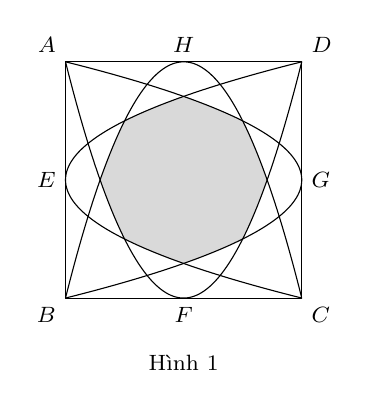
\begin{tikzpicture}[line cap=round, line join=round, >=stealth, font=\footnotesize, scale=1.5]
			% Định nghĩa tọa độ các điểm 
			\coordinate (A) at (-1,1);
			\coordinate (B) at (-1,-1);
			\coordinate (C) at (1,-1);
			\coordinate (D) at (1,1);
			\coordinate (E) at (-1,0);
			\coordinate (F) at (0,-1);
			\coordinate (G) at (1,0);
			\coordinate (H) at (0,1);
			
			% Tô màu phần giao của 4 parabol bằng kỹ thuật clip (tối ưu bằng phép quay)
			\begin{scope}
				\foreach \g in {0, 90, 180, 270} {
					\clip[rotate=\g] (-1,-1) -- plot[domain=-1:1, samples=100] (\x, {1-2*\x*\x}) -- cycle;
				}
				\fill[gray!30] (B) rectangle (D);
			\end{scope}
			
			% Vẽ 4 đường parabol
			\foreach \g in {0, 90, 180, 270} {
				\draw[rotate=\g, domain=-1:1, samples=100, smooth] plot (\x, {1-2*\x*\x});
			}
			
			% Vẽ viền hình vuông ABCD
			\draw (B) rectangle (D);
			
			% Gán nhãn 
			\foreach \p/\anch in {A/above left, B/below left, C/below right, D/above right, E/left, F/below, G/right, H/above} {
				\node[\anch] at (\p) {$\p$};
			}
			
			% Ghi chú tên hình
			\node[below] at (0,-1.4) {Hình $1$};
		\end{tikzpicture}
	}	
	Bước $1$. Vẽ hình vuông $ABCD$ có độ dài cạnh bằng $2$ và lấy trung điểm của $4$ cạnh lần lượt là $E, F, G, H$.\\	
	Bước $2$. Vẽ đồ thị của các hàm bậc hai đi qua $3$ điểm $B, C, H$ và hàm bậc hai đi qua $3$ điểm $F, D, A$.\\	
	Bước $3$. Tương tự như Bước $2$, vẽ đồ thị của các hàm bậc hai đi qua $3$ điểm $A, B, G$ và $3$ điểm $C, D, E$.\\	
	Biết rằng Diện tích phần tô đen trong Hình $1$ được cho bởi công thức $\dfrac{p\sqrt{2} + q}{3}$.\\	
	Hãy tính giá trị của $p - 3q$ (với $p, q$ là các số nguyên).
	
	\shortans{$29$}
	\loigiai{		
			Chọn hệ trục tọa độ $Oxy$ với $O$ là giao điểm của $2$ đường chéo $AC$ và $BD$. Trục $Ox \equiv EG$, trục $Oy \equiv HF$.
			
			\begin{center}
				\begin{tikzpicture}[,line cap=round, line join=round, >=stealth, font=\footnotesize, scale=1.5]
					% 1. ĐỊNH NGHĨA TỌA ĐỘ CÁC ĐIỂM
					\coordinate (A) at (-1,1);
					\coordinate (B) at (-1,-1);
					\coordinate (C) at (1,-1);
					\coordinate (D) at (1,1);
					\coordinate (E) at (-1,0);
					\coordinate (F) at (0,-1);
					\coordinate (G) at (1,0);
					\coordinate (H) at (0,1);
					\coordinate (O) at (0,0);
					\coordinate (N) at (0.5,-0.5);
					\coordinate (M) at (0.5,0);
					\coordinate (P) at ({1/sqrt(2)}, 0); 
					
					\coordinate (I1) at (0.5,0.5);
					\coordinate (I2) at (-0.5,0.5);
					\coordinate (I3) at (-0.5,-0.5);
					
					% 2. TÔ MÀU CÁC VÙNG DIỆN TÍCH
					\begin{scope}
						\foreach \g in {0, 90, 180, 270} {
							\clip[rotate=\g] (-1,-1) -- plot[domain=-1:1, samples=100] (\x, {1-2*\x*\x}) -- cycle;
						}
						\fill[gray!30] (B) rectangle (D);
					\end{scope}
					
					\fill[orange!50] (O) -- (M) -- (N) -- cycle;
					\fill[green!60] (M) -- (N) plot[domain=0.5:1/sqrt(2), samples=100] (\x, {2*\x*\x-1}) -- cycle;
					\fill[green!60] (M) -- (N) -- (P) -- cycle;
					
					% 3. VẼ CÁC ĐƯỜNG CONG VÀ HÌNH CƠ BẢN
					\foreach \g in {0, 90, 180, 270} {
						\draw[gray!80!black, rotate=\g, domain=-1:1, samples=100, smooth] plot (\x, {1-2*\x*\x});
					}
					\draw[black] (B) rectangle (D);
					\draw[blue!70!black] (A) -- (C);
					\draw[blue!70!black] (B) -- (D);
					\draw[black] (M) -- (N);
					
					% 4. VẼ HỆ TRỤC TỌA ĐỘ
					\draw[->, black] (-1.3,0) -- (1.4,0) node[above] {$x$};
					\draw[->, black] (0,-1.3) -- (0,1.4) node[left] {$y$};
					
					% 5. GÁN NHÃN VÀ CHẤM ĐIỂM
					\foreach \p/\anch in {A/above left, B/below left, C/below right, D/above right, E/above left, F/below right, G/above right, H/above right, N/below, O/above left} {
						\fill[black] (\p) circle (0.9pt);
						\node[\anch] at (\p) {$\p$};
					}
					\fill[black] (M) circle (0.9pt);
					\node[above] at (M) {$\dfrac{1}{2}$};
					\foreach \p in {I1, I2, I3} {
						\fill[black] (\p) circle (0.9pt);
					}
				\end{tikzpicture}				
			\end{center}			
			Ta suy ra được phương trình đường chéo $AC \colon y = -x$ và đồ thị hàm số bậc hai đi qua $F, D, A$ là $(P) \colon y = 2x^2 - 1$.			
			Xét phương trình hoành độ giao điểm của đường thẳng $AC$ và parabol $(P)$
			\allowdisplaybreaks 
			\begin{eqnarray*} 
				2x^2 + x - 1 = 0 \Leftrightarrow \hoac{&x = -1 \\ &x = \dfrac{1}{2}.}
			\end{eqnarray*} 			
			Gọi $S_1$ là diện tích hình phẳng giới hạn bởi parabol và trục $Ox$ trên đoạn $\left[\dfrac{1}{2}; \dfrac{1}{\sqrt{2}}\right]$, ta có
			\allowdisplaybreaks 
			\begin{eqnarray*} 
				S_1 &=& \displaystyle\int\limits_{1/2}^{1/\sqrt{2}} (1 - 2x^2) \mathrm{\,d}x = \left. \left( x - \dfrac{2}{3}x^3 \right) \right|_{1/2}^{1/\sqrt{2}} \\
				&=& \dfrac{\sqrt{2}}{3} - \dfrac{5}{12}.			\end{eqnarray*} 				
		Diện tích tam giác giới hạn bởi $y = -x, x = \dfrac{1}{2}$ và trục $Ox$ là $S_2 = \dfrac{1}{8}$.\\		
		Do tính đối xứng, diện tích phần tô màu đen của toàn bộ Hình $1$ là
		\allowdisplaybreaks 
		\begin{eqnarray*} 
			S = 8(S_1 + S_2) = 8\left( \dfrac{\sqrt{2}}{3} - \dfrac{5}{12} + \dfrac{1}{8} \right) = \dfrac{8\sqrt{2} - 7}{3}.
		\end{eqnarray*} 
		
		Đồng nhất hệ số ta được $p = 8, q = -7 \Rightarrow p - 3q = 8 - 3(-7) = 29$.
	}
\end{ex}

%%%%%-----Câu 3-----%%%%%
\begin{ex}%[Sở GD\&ĐT THANH HÓA, TRƯỜNG THPT YÊN ĐỊNH 1]%[Trần Tiến Sĩ, 26-2-DuAnDeTHPT-2025-2026]%[1H8V6-5]
	Cho hình chóp $S.ABC$ có đáy $ABC$ là tam giác vuông tại $A$, $AC = 10\sqrt{3}$, góc $\widehat{ABC} = 30^\circ$, góc giữa $SC$ và mặt phẳng $(ABC)$ bằng $60^\circ$. Cạnh bên $SA$ vuông góc với đáy. Tính khoảng cách từ điểm $A$ đến mặt phẳng $(SBC)$ (làm tròn kết quả đến hàng phần chục).
	\shortans{$13{,}4$}
	\loigiai{
		\immini{
			Kẻ $AE \perp BC$ tại $E$, $AK \perp SE$ tại $K$. \\			
			Ta có $BC \perp AE$ và $BC \perp SA \Rightarrow BC \perp (SAE) \Rightarrow BC \perp AK$.\\			
			Mà $AK \perp SE \Rightarrow AK \perp (SBC)$. Vậy $d(A, (SBC)) = AK$.\\			
			Xét tam giác $ABC$ vuông tại $A$, có $\widehat{ABC} = 30^\circ$, $AC = 10\sqrt{3}$.\\			
			$AB = \dfrac{AC}{\tan 30^\circ} = \dfrac{10\sqrt{3}}{\dfrac{1}{\sqrt{3}}} = 30$.\\		
			Xét  tam giác vuông $ABC$ có đường cao $ \dfrac{1}{AE^2} = \dfrac{1}{AB^2} + \dfrac{1}{AC^2} \Rightarrow AE = 15$.\\			
			Góc giữa $SC$ và mặt phẳng $(ABC)$ là $\widehat{SCA} = 60^\circ$.\\			
			Xét tam giác vuông $SAC \colon SA = AC \tan 60^\circ = 10\sqrt{3} \cdot \sqrt{3} = 30$.\\			
			Xét tam giác vuông $SAE$
			\allowdisplaybreaks 
			\begin{eqnarray*} 
				&AK = \dfrac{SA \cdot AE}{\sqrt{SA^2 + AE^2}} = \dfrac{30 \cdot 15}{\sqrt{30^2 + 15^2}} = \dfrac{30}{\sqrt{5}} \approx 13{,}4.
			\end{eqnarray*} 
		}{
			\begin{tikzpicture}[,line cap=round, line join=round, scale=0.75, font=\footnotesize]
				% Khai báo tọa độ các đỉnh
				\coordinate (A) at (0,0);
				\coordinate (B) at (-1.2,-2.5);
				\coordinate (C) at (5,0);
				\coordinate (S) at (0,3.5);
				
				\coordinate (E) at ($(B)!0.4!(C)$);
				\coordinate (K) at ($(S)!0.55!(E)$);
				
				% Macro vẽ góc vuông nhanh
				\tikzset{
					ra/.style n args={3}{
						insert path={
							($(#2)!2mm!(#1)$) -- ($($(#2)!2mm!(#1)$)+($(#2)!2mm!(#3)$)-(#2)$) -- ($(#2)!2mm!(#3)$)
						}
					}
				}
				% Vẽ các đường đứt nét
				\draw[dashed] (S)--(A);
				\draw[dashed] (A)--(B);
				\draw[dashed] (A)--(C);
				\draw[dashed] (A)--(E);
				\draw[red, dashed] (A)--(K);
				
				% Vẽ các đường liền nét
				\draw[] (S)--(B)--(C)--cycle;
				\draw[] (S)--(E);
				
				% Vẽ các điểm chấm đen tại đỉnh
				\foreach \p in {S, A, B, C, E, K} {
					\fill[black] (\p) circle (1.2pt);
				}
				% Vẽ các ký hiệu góc vuông
				\draw [ra={C}{E}{A}];
				\draw [ra={S}{A}{B}];
				\draw [ra={S}{A}{C}];
				\draw [ra={A}{K}{S}];
				
				% Gán nhãn các điểm
				\node[above] at (S) {$S$};
				\node[left] at (A) {$A$};
				\node[below left] at (B) {$B$};
				\node[right] at (C) {$C$};
				\node[below right ] at (E) {$E$};
				\node[right] at (K) {$K$};
			\end{tikzpicture}
		}
	}
\end{ex}

%%%%%-----Câu 4-----%%%%%
\begin{ex}%[Sở GD\&ĐT THANH HÓA, TRƯỜNG THPT YÊN ĐỊNH 1]%[Trần Tiến Sĩ, 26-2-DuAnDeTHPT-2025-2026]%[2D1V3-6]
	Một hộ gia đình chuyên làm thịt trâu sấy khô để bán, mỗi ngày hộ đó sản xuất được $x$ kg thịt, $(1 \le x \le 20)$. Tổng chi phí sản xuất $x$ kg thịt trâu khô, tính bằng nghìn đồng, cho bởi hàm chi phí $C(x) = x^3 - 9x^2 + 345x + 450$. Giả sử hộ gia đình này bán hết số thịt làm ra mỗi ngày với giá $750$ nghìn đồng/kg. Gọi $L(x)$ là lợi nhuận thu được khi bán $x$ kg thịt trâu sấy khô. Hỏi lợi nhuận tối đa mà hộ gia đình này thu được trong một ngày (kết quả tính theo đơn vị nghìn đồng)?
	\shortans{$4275$}
	\loigiai{
		Số tiền thu về khi bán $x$ kg thịt trâu khô là $750x$ (nghìn đồng).\\		
		Lợi nhuận thu được khi bán $x$ kg thịt là
		\allowdisplaybreaks 
		\begin{eqnarray*} 
			L(x) &=& 750x - (x^3 - 9x^2 + 345x + 450) \\
			&=& -x^3 + 9x^2 + 405x - 450, 
		\end{eqnarray*} 
		với $x \in [1; 20]$.\\		
		Ta có đạo hàm $L'(x) = -3x^2 + 18x + 405$.
		\allowdisplaybreaks 
		\begin{eqnarray*} 
			L'(x) = 0 \Leftrightarrow \hoac{&x = 15 \in [1; 20] \\ &x = -9 \notin [1; 20].}
		\end{eqnarray*} 		
		Lập bảng biến thiên của hàm số $y= L(x)$ trên đoạn $[1; 20]$
		\begin{center}
			
\begin{tikzpicture}
				\tkzTabInit[nocadre=false,lgt=1.2,espcl=3.5,deltacl=0.6]
				{$x$ / 1, $L'(x)$ / 1, $L(x)$ / 2}
				{$1$, $15$, $20$}
				\tkzTabLine{ , +, 0, -, }
				\tkzTabVar{-/ $-37$, +/ $4275$, -/ $3250$}
			\end{tikzpicture}
		\end{center}
		Ta thấy hàm số đạt giá trị lớn nhất tại $x = 15$.	Khi đó $L(15) = 4275$.\\
		
		Vậy lợi nhuận tối đa hộ gia đình thu được trong $1$ ngày là $4275$ nghìn đồng.
	}
\end{ex}
%%%%%-----Câu 5-----%%%%%
\begin{ex}%[Sở GD\&ĐT THANH HÓA, TRƯỜNG THPT YÊN ĐỊNH 1]%[Trần Tiến Sĩ, 26-2-DuAnDeTHPT-2025-2026]%[2H5C3-2]
	Trong không gian với hệ tọa độ $Oxyz$, cho $2$ điểm $A(5;0;0), B(4;3;0)$ và điểm $C$ nằm trên trục $Oz$. Gọi $H$ là trực tâm tam giác $ABC$. Khi $C$ di chuyển trên trục $Oz$ thì $H$ luôn thuộc một đường tròn cố định. Tính bán kính của đường tròn đó (kết quả làm tròn đến hàng phần trăm).
	\shortans{$0{,}26$}
	\loigiai{
		
			\begin{center}
				\begin{tikzpicture}[ line cap=round, line join=round, scale=0.85, font=\footnotesize]
					
					% 1. Khai báo tọa độ các đỉnh chính (Thuần 2D)
					\coordinate (O) at (0,0);
					\coordinate (A) at (-2.5,-3.5);
					\coordinate (B) at (6.5,-1.5);
					\coordinate (C) at (0,5);
					
					% 2. Lấy các điểm E, K, H theo tham số tỉ lệ
					\coordinate (E) at ($(A)!0.5!(B)$);
					\coordinate (K) at ($(O)!0.6!(E)$);
					\coordinate (H) at ($(C)!0.75!(E)$);
					
					% Lấy chân các đường cao bằng lệnh giao điểm
					\coordinate (Pa) at (intersection of B--K and O--A);
					\coordinate (Pb) at (intersection of A--K and O--B);
					\coordinate (Pbc) at (intersection of A--H and C--B);
					\coordinate (Pac) at (intersection of B--H and C--A);
					
					% Đầu mút các trục tọa độ
					\coordinate (Ax) at ($(O)!1.2!(A)$);
					\coordinate (Ay) at (5,0);
					\coordinate (Az) at (0,6);
					
					% Macro vẽ góc vuông nhanh
					\tikzset{
						ra/.style n args={3}{
							insert path={
								($(#2)!2mm!(#1)$) -- ($($(#2)!2mm!(#1)$)+($(#2)!2mm!(#3)$)-(#2)$) -- ($(#2)!2mm!(#3)$)
							}
						}
					}
					
					% 3. Vẽ các trục tọa độ
					\draw[dashed] (O) -- (A);
					\draw[->] (A) -- (Ax) node[left] {$x$};
					
					\draw[dashed] (O) -- (C);
					\draw[->] (C) -- (Az) node[above] {$z$};
					
					\draw[dashed] (O) -- (Ay);
					\draw[->] (Ay) -- ($(Ay)+(2.5,0)$) node[right] {$y$};
					
					% 4. Vẽ các đường đứt nét (cạnh khuất và đường phụ)
					\draw[dashed] (O) -- (B);
					\draw[dashed] (O) -- (E);
					\draw[dashed] (K) -- (H);
					\draw[dashed] (A) -- (Pb);
					\draw[dashed] (B) -- (Pa);
					
					% 5. Vẽ các đường liền nét (cạnh thấy)
					\draw (A) -- (B) -- (C) -- cycle; 
					\draw (C) -- (E);
					\draw (A) -- (Pbc);
					\draw (B) -- (Pac);
					
					% 6. Vẽ các ký hiệu góc vuông
					\draw [ra={C}{E}{B}];
					\draw [ra={O}{E}{A}];
					\draw [ra={A}{Pbc}{B}];
					\draw [ra={B}{Pac}{A}];
					\draw [ra={B}{Pa}{O}];
					\draw [ra={A}{Pb}{O}];
					\draw [ra={K}{H}{C}];
					
					% 7. Chấm các điểm phụ (chân đường cao)
					\foreach \p in {Pa, Pb, Pbc, Pac} {
						\fill (\p) circle (1.2pt); 
					}
					
					% 8. Chấm và gán nhãn các đỉnh chính bằng vòng lặp
					\foreach \p/\anch in {O/left, A/left, B/right, C/left, E/below, K/below, H/above right} {
						\fill (\p) circle (1.2pt);
						\node[\anch] at (\p) {$\p$};
					}
					
				\end{tikzpicture}
			\end{center}			
			Ta có $OA = OB = 5$ nên tam giác $OAB$ cân tại $O$. Điểm $C$ nằm trên trục $Oz \Rightarrow C(0; 0; c)$.\\			
			Gọi $E\left(\dfrac{9}{2}; \dfrac{3}{2}; 0\right)$ là trung điểm của $AB$. \\			
			Do $\heva{&AB \perp OC \\ &AB \perp OE}\Rightarrow AB \perp (OCE)$.\\			
			Mặt phẳng $(OCE)$ cố định vuông góc với $AB$. Mà $H$ là trực tâm tam giác $ABC$ nên $H \in (OCE)$.\\			
			Gọi $K(a; b; 0)$ là trực tâm tam giác $OAB$ (do $K \in (Oxy)$).\\			
			Ta có hệ phương trình
			\allowdisplaybreaks 
			\begin{eqnarray*} 
				\heva{&\vec{OK} \cdot \vec{AB} = 0 \\ &\vec{BK} \cdot \vec{OA} = 0} \Leftrightarrow \heva{&-a + 3b = 0 \\ &5(a-4) = 0}  \Leftrightarrow \heva{&a = 4 \\ &b = \dfrac{4}{3}}
			\end{eqnarray*} 
			Suy ra $K\left(4; \dfrac{4}{3}; 0\right)$.\\			
			Ta chứng minh được $KH \perp (CAB)$ (do $AB \perp (OEC) \Rightarrow AB \perp HK$ và $CA \perp (BHK) \Rightarrow CA \perp HK$).
			Suy ra $\widehat{KHE} = 90^\circ$.\\			
			Điểm $H$ luôn nhìn đoạn $KE$ dưới một góc vuông.
			Do đó $H$ luôn thuộc một đường tròn cố định là giao tuyến của mặt cầu đường kính $KE$ và mặt phẳng $(OCE)$.\\			
			Bán kính đường tròn đó là $R = \dfrac{KE}{2} = \dfrac{1}{2}\sqrt{\left(\dfrac{9}{2} - 4\right)^2 + \left(\dfrac{3}{2} - \dfrac{4}{3}\right)^2} = \dfrac{\sqrt{10}}{12} \approx 0{,}26$.		
	}
\end{ex}

%%%%%-----Câu 6-----%%%%%
\begin{ex}%[Sở GD\&ĐT THANH HÓA, TRƯỜNG THPT YÊN ĐỊNH 1]%[Trần Tiến Sĩ, 26-2-DuAnDeTHPT-2025-2026]%[0D2V2-3]
	Bác Bình có một mảnh đất rộng $6$ ha. Bác dự tính trồng cà chua và bắp cho mùa vụ sắp tới. Nếu trồng bắp thì bác Bình cần $10$ ngày để trồng $1$ ha. Nếu trồng cà chua thì bác Bình cần $20$ ngày để trồng $1$ ha. Biết rằng mỗi ha bắp sau thu hoạch bán được $30$ triệu đồng, mỗi ha cà chua sau thu hoạch bán được $50$ triệu đồng và bác Bình chỉ còn $100$ ngày để canh tác cho kịp mùa vụ. Số tiền nhiều nhất mà bác Bình có thể thu được sau mùa vụ này là bao nhiêu (kết quả theo đơn vị triệu đồng)?
	\shortans{$260$}
	\loigiai{
		\immini{
			Gọi diện tích bác Bình trồng bắp là $x$ (ha), diện tích trồng cà chua là $y$ (ha) ($x \ge 0, y \ge 0$).
			
			Tổng diện tích không quá $6$ ha nên $x + y \le 6$.
			
			Tổng số ngày công trồng bắp là $10x$, số ngày công trồng cà chua là $20y$. Do chỉ có $100$ ngày nên $10x + 20y \le 100 \Leftrightarrow x + 2y \le 10$.
			
			Số tiền thu được là hàm mục tiêu $T(x,y) = 30x + 50y$ (triệu đồng).
			
			Hệ bất phương trình ràng buộc
			\allowdisplaybreaks 
			\begin{eqnarray*} 
				\heva{&x \ge 0 \\ &y \ge 0 \\ &x + y \le 6 \\ &x + 2y \le 10.}
			\end{eqnarray*} 
		}{
			\begin{tikzpicture}[ line cap=round, line join=round, >=stealth, font=\footnotesize, scale=0.8]
				
				% Cắt xén khung hình để đồ thị hiển thị vừa vặn
				\clip (-1.5,-1.5) rectangle (7.5, 6.5);
				
				% 1. ĐỊNH NGHĨA TỌA ĐỘ CÁC ĐỈNH MIỀN NGHIỆM
				\coordinate (A) at (0,0); % A trùng O
				\coordinate (B) at (0,5);
				\coordinate (C) at (2,4);
				\coordinate (D) at (6,0);
				
				% 2. TÔ MÀU MIỀN KHÔNG THỎA MÃN (GẠCH CHÉO)
				\fill[pattern=north east lines, pattern color=gray!80] (-2,-2) rectangle (8,8);
				\fill[white] (A) -- (B) -- (C) -- (D) -- cycle;
				
				% 3. VẼ LƯỚI TỌA ĐỘ
				\draw[dotted, gray!60, step=1] (-1.5,-1.5) grid (7.5,6.5);
				
				% 4. VẼ HỆ TRỤC TỌA ĐỘ
				\draw[->, ] (-1.5,0) -- (7.5,0) node[above left] {$x$};
				\draw[->, ] (0,-1.5) -- (0,6.5) node[below right] {$y$};
				
				% 5. VẼ CÁC ĐƯỜNG BIÊN CỦA HỆ BẤT PHƯƠNG TRÌNH
				% Đường x + y = 6
				\draw[] (-1,7) -- (7,-1);
				% Đường x + 2y = 10
				\draw[] (-2,6) -- (8,1);
				
				% 6. CHẤM ĐỈNH VÀ GÁN NHÃN 
				% Xử lý riêng gốc tọa độ để tách 2 nhãn O và A
				\fill[black] (A) circle (1.2pt);
				\node[below left] at (A) {$O$};
				\node[right] at (1,5) {$d_1 \colon x+y=6$};
				\node[] at (3,1) {$d_2 \colon x+2y=10$};
				\node[below left] at (B) {$C$};
				\node[below left] at (C) {$B$};
				\node[below left] at (D) {$A$};
				
				\foreach \p/\anch in {B/below left, C/below left, D/below left} {
					\fill[black] (\p) circle (1.2pt);
				
				}
				
			\end{tikzpicture}
		}
		Miền nghiệm của hệ là một đa giác có các đỉnh $O(0;0), A(6;0), B(2;4), C(0;5)$.\\		
		Lần lượt thay tọa độ các đỉnh vào hàm $T$ ta được
		\allowdisplaybreaks 
		\begin{eqnarray*} 
			T(0,0) &=& 0\\
			T(6,0) &=& 30(6) + 0 = 180\\
			T(2,4) &=& 30(2) + 50(4) = 260\\
			T(0,5) &=& 50(5) = 250.
		\end{eqnarray*} 		
		Giá trị lớn nhất đạt được là $260$ tại $x=2, y=4$.\\		
		Vậy số tiền lớn nhất bác Bình thu được là $260$ triệu đồng.
		
	}
\end{ex}

\Closesolutionfile{ans}
